%%%%%%%%%%%%%%%%%%%%%%%%%%%%%%%%%%%%%%%%%
% Beamer Presentation
% LaTeX Template
% Version 1.0 (10/11/12)
%
% This template has been downloaded from:
% http://www.LaTeXTemplates.com
%
% License:
% CC BY-NC-SA 3.0 (http://creativecommons.org/licenses/by-nc-sa/3.0/)
%
%%%%%%%%%%%%%%%%%%%%%%%%%%%%%%%%%%%%%%%%%

%----------------------------------------------------------------------------------------
%	PACKAGES AND THEMES
%----------------------------------------------------------------------------------------

\documentclass[10pt]{beamer}

\mode<presentation> {
	
	% The Beamer class comes with a number of default slide themes
	% which change the colors and layouts of slides. Below this is a list
	% of all the themes, uncomment each in turn to see what they look like.
	
	%\usetheme{default}
	%\usetheme{AnnArbor}
	%\usetheme{Antibes}
	%\usetheme{Bergen}
	%\usetheme{Berkeley}
	%\usetheme{Berlin}
	%\usetheme{Boadilla}
	%\usetheme{CambridgeUS}
	%\usetheme{Copenhagen}
	%\usetheme{Darmstadt}
	%\usetheme{Dresden}
	%\usetheme{Frankfurt}
	%\usetheme{Goettingen}
	%\usetheme{Hannover}
	%\usetheme{Ilmenau}
	%\usetheme{JuanLesPins}
	%\usetheme{Luebeck}
	\usetheme{Madrid}
	%\usetheme{Malmoe}
	%\usetheme{Marburg}
	%\usetheme{Montpellier}
	%\usetheme{PaloAlto}
	%\usetheme{Pittsburgh}
	%\usetheme{Rochester}
	%\usetheme{Singapore}
	%\usetheme{Szeged}
	%\usetheme{Warsaw}
	
	% As well as themes, the Beamer class has a number of color themes
	% for any slide theme. Uncomment each of these in turn to see how it
	% changes the colors of your current slide theme.
	
	%\usecolortheme{albatross}
	\usecolortheme{beaver}
	%\usecolortheme{beetle}
	%\usecolortheme{crane}
	%\usecolortheme{dolphin}
	%\usecolortheme{dove}
	%\usecolortheme{fly}
	%\usecolortheme{lily}
	%\usecolortheme{orchid}
	%\usecolortheme{rose}
	%\usecolortheme{seagull}
	%\usecolortheme{seahorse}
	%\usecolortheme{whale}
	%\usecolortheme{wolverine}
	
	\usefonttheme{serif}
	
	%\setbeamertemplate{footline} % To remove the footer line in all slides uncomment this line
	%\setbeamertemplate{footline}[page number] % To replace the footer line in all slides with a simple slide count uncomment this line
	
	%\setbeamertemplate{navigation symbols}{} % To remove the navigation symbols from the bottom of all slides uncomment this line
}
\usepackage{ragged2e}
\usepackage{lipsum}
\usepackage{amsmath}
\usepackage{gensymb}
\usepackage{textcomp}
\usepackage{braket}
\usepackage{lipsum}
\usepackage{bm}
\usepackage{graphicx, float} % Allows including images
\usepackage[centerlast]{subfigure}
\usepackage{wrapfig}
\usepackage{booktabs} % Allows the use of \toprule, \midrule and \bottomrule in tables
\usepackage{multicol}
\usepackage{multirow}
\usepackage[font=scriptsize,labelfont=scriptsize]{caption}
\usepackage[spanish,es-tabla]{babel}
\usepackage[utf8]{inputenc}
\usepackage{csquotes}
\spanishdecimal{.}
\usepackage{gensymb}
\usepackage{textcomp}
\usepackage{amsmath}
\usepackage{nicefrac}

\usepackage{listings}
\usepackage{xcolor}

\usepackage{hyperref}
\hypersetup{
    colorlinks=true,
    linkcolor=black,
    filecolor=black,      
    urlcolor=blue,
    citecolor=black,
}
\urlstyle{same}

\definecolor{codegreen}{rgb}{0,0.6,0}
\definecolor{codegray}{rgb}{0.5,0.5,0.5}
\definecolor{codepurple}{rgb}{0.58,0,0.82}
\definecolor{backcolour}{rgb}{0.95,0.95,0.92}
\definecolor{codeblue}{RGB}{0, 180,201}
\definecolor{codered}{RGB}{238,25,0}



\lstdefinestyle{mystyle}{
	backgroundcolor=\color{backcolour},   
	commentstyle=\color{codeblue},
	keywordstyle=\color{codegreen},
	%numberstyle=\tiny\color{codegray},
	stringstyle=\color{codepurple},
	basicstyle=\ttfamily\footnotesize,
	breakatwhitespace=false,         
	breaklines=true,                 
	captionpos=b,                    
	keepspaces=true,                 
	%numbers=left,                    
	%numbersep=5pt,                  
	showspaces=false,                
	showstringspaces=false,
	showtabs=false,                  
	tabsize=2,
	moredelim=**[s][\color{codered}]{"""}{"""}
}

\lstset{emph={%  
		USE, KEYSPACE, WITH%
	},emphstyle={\color{codegreen}}%
}%

\lstset{literate = {á}{{\'a}}1 {é}{{\'e}}1 {í}{{\'i}}1 {Í}{{\'I}}1 {ó}{{\'o}}1 {ú}{{\'u}}1 {ñ}{{\~n}}1 {°}{{\textdegree}}1 {means-mu}{{$\mu$}}1 {std-sigma}{{$\sigma$}}1}

\lstset{language=Python, style=mystyle}

\newcommand\blfootnote[1]{%
  \begingroup
  \renewcommand\thefootnote{}\footnote{#1}%
  \addtocounter{footnote}{-1}%
  \endgroup
}

\setbeamertemplate{caption}[numbered]
%\captionsetup[figure]{font=scriptsize,labelfont=footnotesize}
%\captionsetup[subfigure]{font=scriptsize,labelfont=scriptsize}


%\makeatletter
%\newcommand\titlegraphicii[1]{\def\inserttitlegraphicii{#1}}
%\titlegraphicii{}
%\setbeamertemplate{title page}
%{
%	\vbox{}
%	{\usebeamercolor[fg]{titlegraphic}\inserttitlegraphic\hfill\inserttitlegraphicii\par}
%	\begin{centering}
%		\begin{beamercolorbox}[sep=8pt,center]{institute}
%			\usebeamerfont{institute}\insertinstitute
%		\end{beamercolorbox}
%		\begin{beamercolorbox}[sep=8pt,center]{title}
%			\usebeamerfont{title}\inserttitle\par%
%			\ifx\insertsubtitle\@empty%
%			\else%
%			\vskip0.25em%
%			{\usebeamerfont{subtitle}\usebeamercolor[fg]{subtitle}\insertsubtitle\par}%
%			\fi%     
%		\end{beamercolorbox}%
%		\vskip1em\par
%		\begin{beamercolorbox}[sep=8pt,center]{date}
%			\usebeamerfont{date}\insertdate
%		\end{beamercolorbox}%\vskip0.5em
%		\begin{beamercolorbox}[sep=8pt,center]{author}
%			\usebeamerfont{author}\insertauthor
%		\end{beamercolorbox}
%	\end{centering}
%	%\vfill
%}
%
%\titlegraphic{
\includegraphics[height=1.5cm,width=2cm]{unam.png}}
%\titlegraphicii{
\includegraphics[height=1.5cm,width=2cm]{unam.png}}

%----------------------------------------------------------------------------------------
%	TITLE PAGE
%----------------------------------------------------------------------------------------
\vspace*{3em}
\title[Shared Task at IberLEF 2021]{EXIST: sEXism Identification in Social neTworks} % The short title appears at the bottom of every slide, the full title is only on the title page

\author[David Guzmán]{E. David Guzmán Ramírez} % Your name
\institute[IIMAS, UNAM] % Your institution as it will appear on the bottom of every slide, may be shorthand to save space
{	Licenciatura en Ciencia de Datos \\
	Minería de Textos \\ \medskip Dra. Helena Gómez Adorno \\ M. en C. Ricardo Montalvo Lezama}
\date{{\tiny 9 de junio de 2021}} % Date, can be changed to a custom date

\vspace*{-5em}

\titlegraphic{
\includegraphics[width=1.8cm]{images/unam.png}\hspace*{7.5cm}~%
	
\includegraphics[width=2.0cm]{images/iimas.png} 
}

\begin{document}
	
	
\begin{frame}
	\titlepage % Print the title page as the first slide
\end{frame}

\begin{frame}
\frametitle{Contenidos}
\justify

\tableofcontents
\end{frame}

\section{Introducción}
\begin{frame}{Introducción}
\justify
\small
\href{http://nlp.uned.es/exist2021/}{EXIST: sEXism Identification in Social neTworks} es una competencia en el marco de \href{https://sites.google.com/view/iberlef2021/home}{IBERLEF 2021} (Iberian Languages Evaluation Forum) para la detección de información dañina. \medskip

De acuerdo al diccionario de Oxford, se entiende como \textbf{sexismo} \emph{los prejuicios, estereotipos o discriminación, generalmente contra las mujeres, en base a su género}. La desigualdad y la discriminación contra las mujeres que siguen arraigadas en nuestra sociedad se reproducen cada vez más en línea. \medskip

\end{frame}


\section{Motivación}
\begin{frame}{Motivación}
\justify
\small
Detectar el sexismo online puede resultar complicado, ya que puede expresarse de formas muy diferentes. El objetivo es la detección del sexismo en un sentido amplio, desde la misoginia explícita hasta otras expresiones sutiles que involucran comportamientos sexistas implícitos. \medskip

La \textbf{identificación automática} de sexismo en un sentido amplio puede ayudar a crear, diseñar y determinar la evolución de nuevas políticas de igualdad, así como fomentar mejores comportamientos en la sociedad.
\end{frame}

\section{Descripción del problema}
\begin{frame}{Descripción del problema}
\justify
\small

Se pedirá a los participantes que clasifiquen \emph{tweets} y \emph{gab}, tanto en inglés como español, de acuerdo con las dos tareas siguientes:

\begin{enumerate}
\item \textbf{Tarea 1: Identificación del sexismo.} Es un problema de clasificación binaria, los sistemas tienen que decidir si un texto dado es sexista o no.

\item \textbf{Tarea 2: Categorización del sexismo.} Una vez que un mensaje ha sido clasificado como sexista, la segunda tarea tiene como objetivo categorizar el mensaje según el tipo de sexismo, de acuerdo a la siguiente clasificación:

\begin{enumerate}
\item Desigualdad.
\item Estereotipos y dominio.
\item Cosificación.
\item Violencia sexual.
\item Misoginia y violencia no sexual.
\end{enumerate}

\end{enumerate}

\end{frame}

\section{Análisis exploratorio}
\begin{frame}{Análisis exploratorio}
\justify	
\small
El conjunto de datos EXIST incorpora cualquier tipo de expresión sexista o fenómenos relacionados, incluidas las afirmaciones descriptivas o informadas donde el mensaje sexista es un informe o una descripción de un comportamiento sexista. \medskip

Los textos fueron extraídos de varias cuentas de Twitter y la red social Gab, estos últimos sólo están en conjunto de prueba para para medir la diferencia entre redes sociales con y sin \emph{control de contenido}.

% Please add the following required packages to your document preamble:
% \usepackage{booktabs}
% \usepackage{graphicx}
\begin{table}[H]
\centering
\resizebox{0.3\textwidth}{!}{%
\begin{tabular}{@{}ccc@{}}
\toprule
\textbf{Datos} & \textbf{Inglés} & \textbf{Español} \\ \midrule
Train          & 3,436           & 3,541            \\
Test           & 2,208           & 2,160            \\ \bottomrule
\end{tabular}%
}
\caption{Cantidad de textos en el conjunto de entrenamiento y prueba.}
\end{table}

\end{frame}

\begin{frame}{Análisis exploratorio}
\justify	
\small

\begin{figure}[H]
\centering
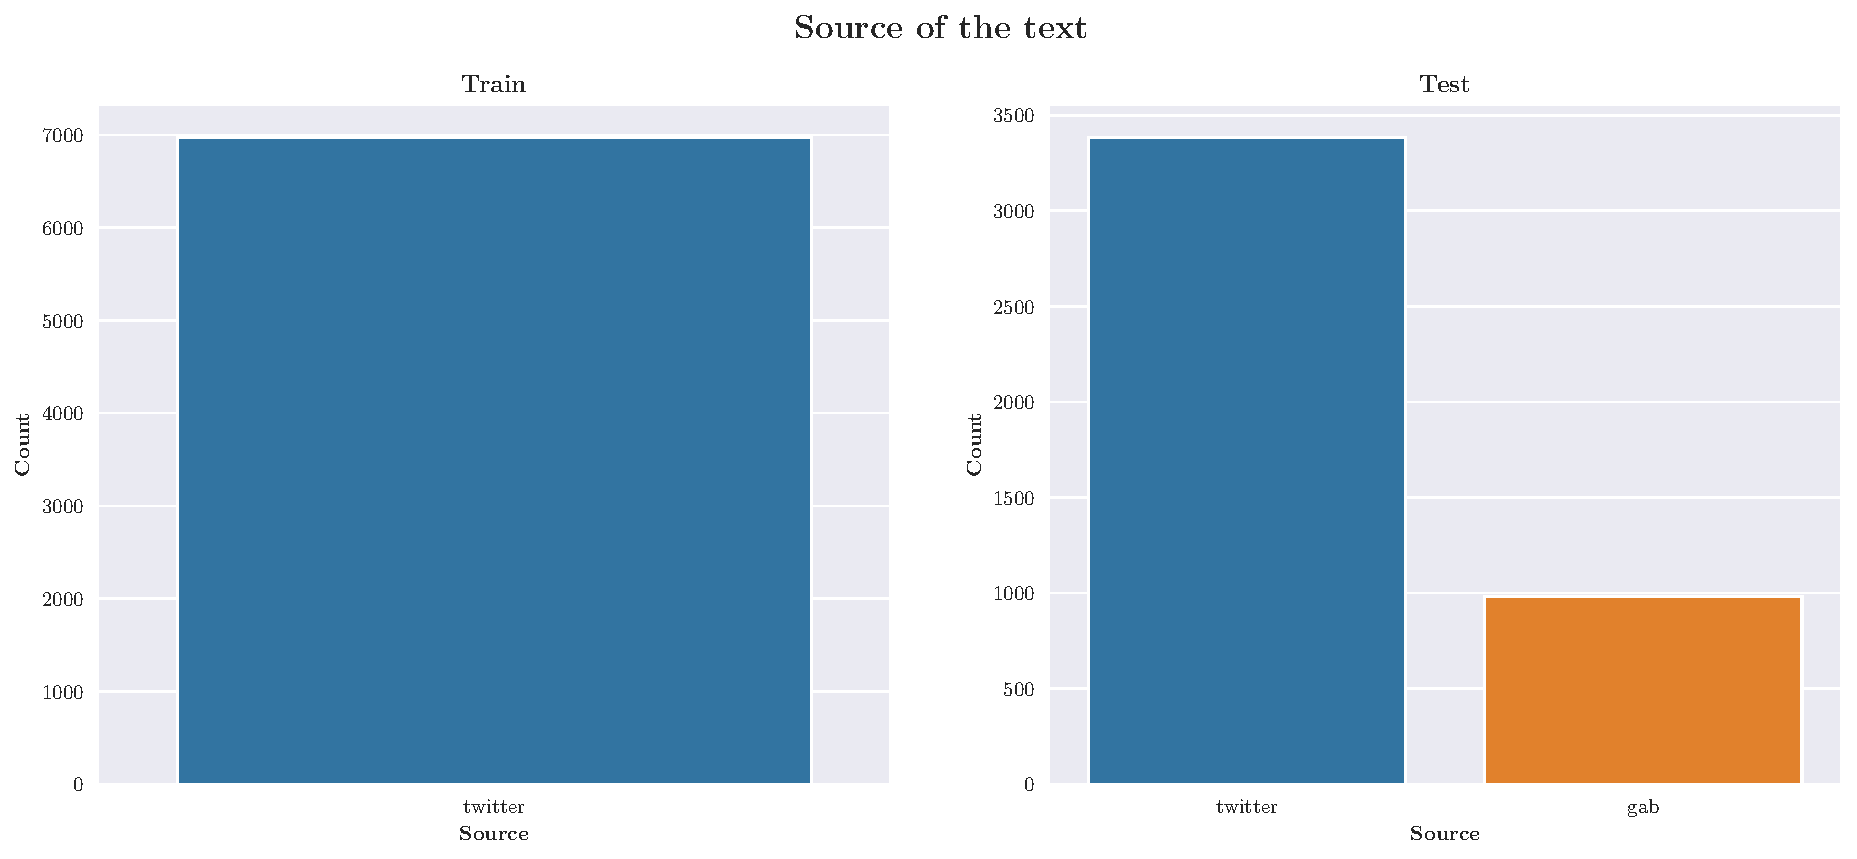
\includegraphics[width=0.8\linewidth]{images/source.pdf}
\caption{Procedencia de los textos en entrenamiento y prueba.}
\end{figure}

\end{frame}

\begin{frame}{Análisis exploratorio}
\justify	
\small

\begin{figure}[H]
\centering
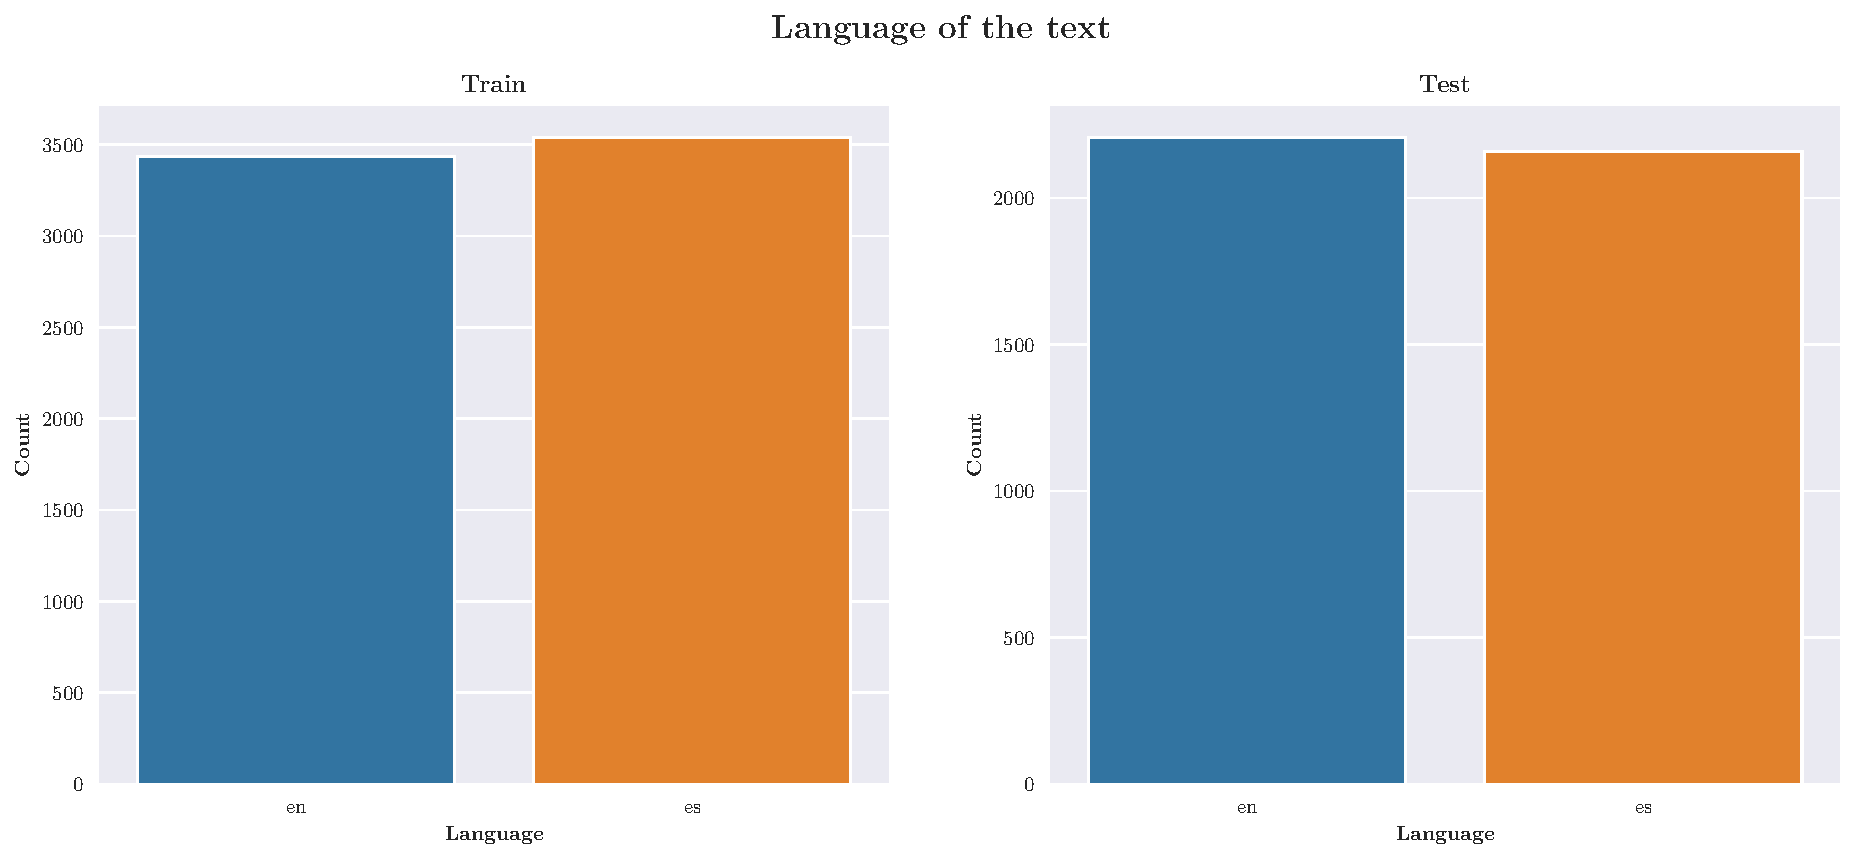
\includegraphics[width=0.8\linewidth]{images/language.pdf}
\caption{Idioma de los textos en entrenamiento y prueba.}
\end{figure}

\end{frame} 

\begin{frame}{Análisis exploratorio}
\justify	
\small

\begin{figure}[H]
\centering
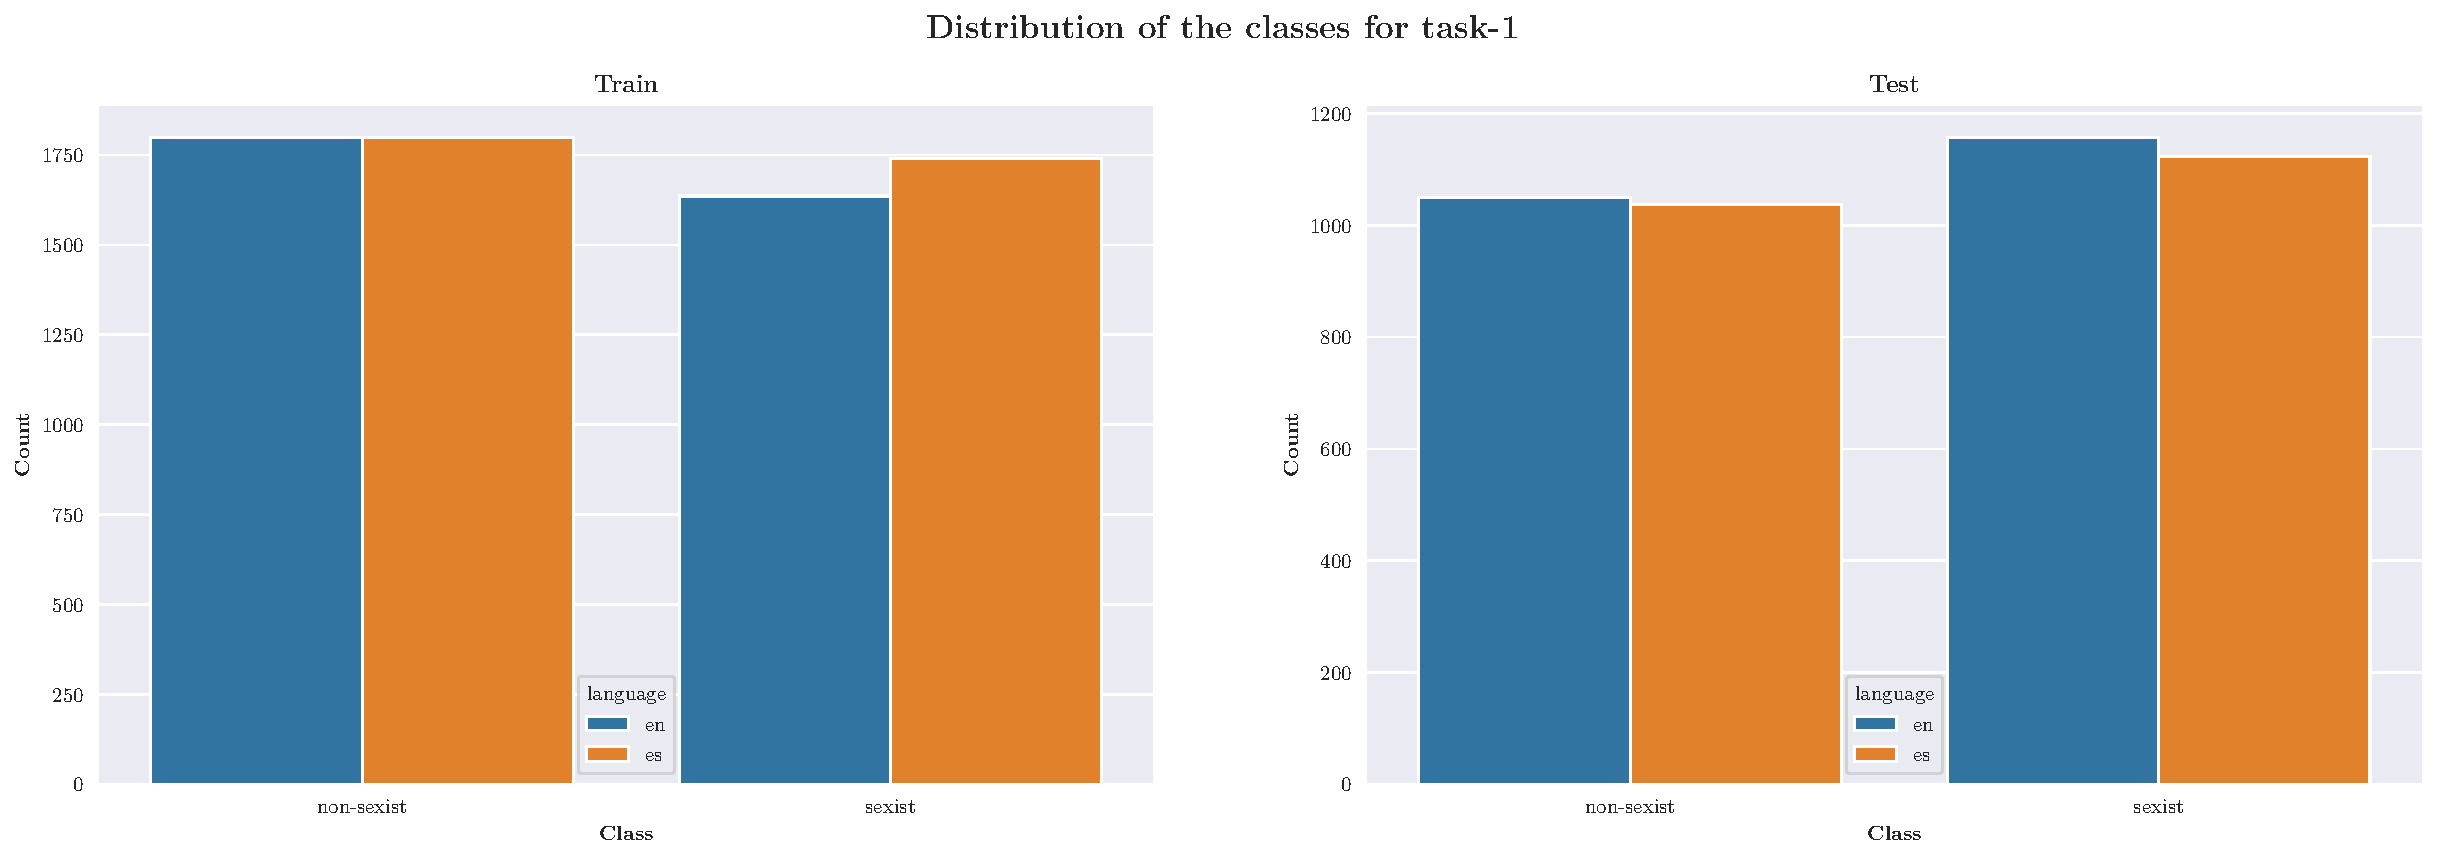
\includegraphics[width=0.8\linewidth]{images/task1.pdf}
\caption{Distribución de las clases en entrenamiento y prueba para la primera tarea.}
\end{figure}

\end{frame} 

\begin{frame}{Análisis exploratorio}
\justify	
\small

\begin{figure}[H]
\centering
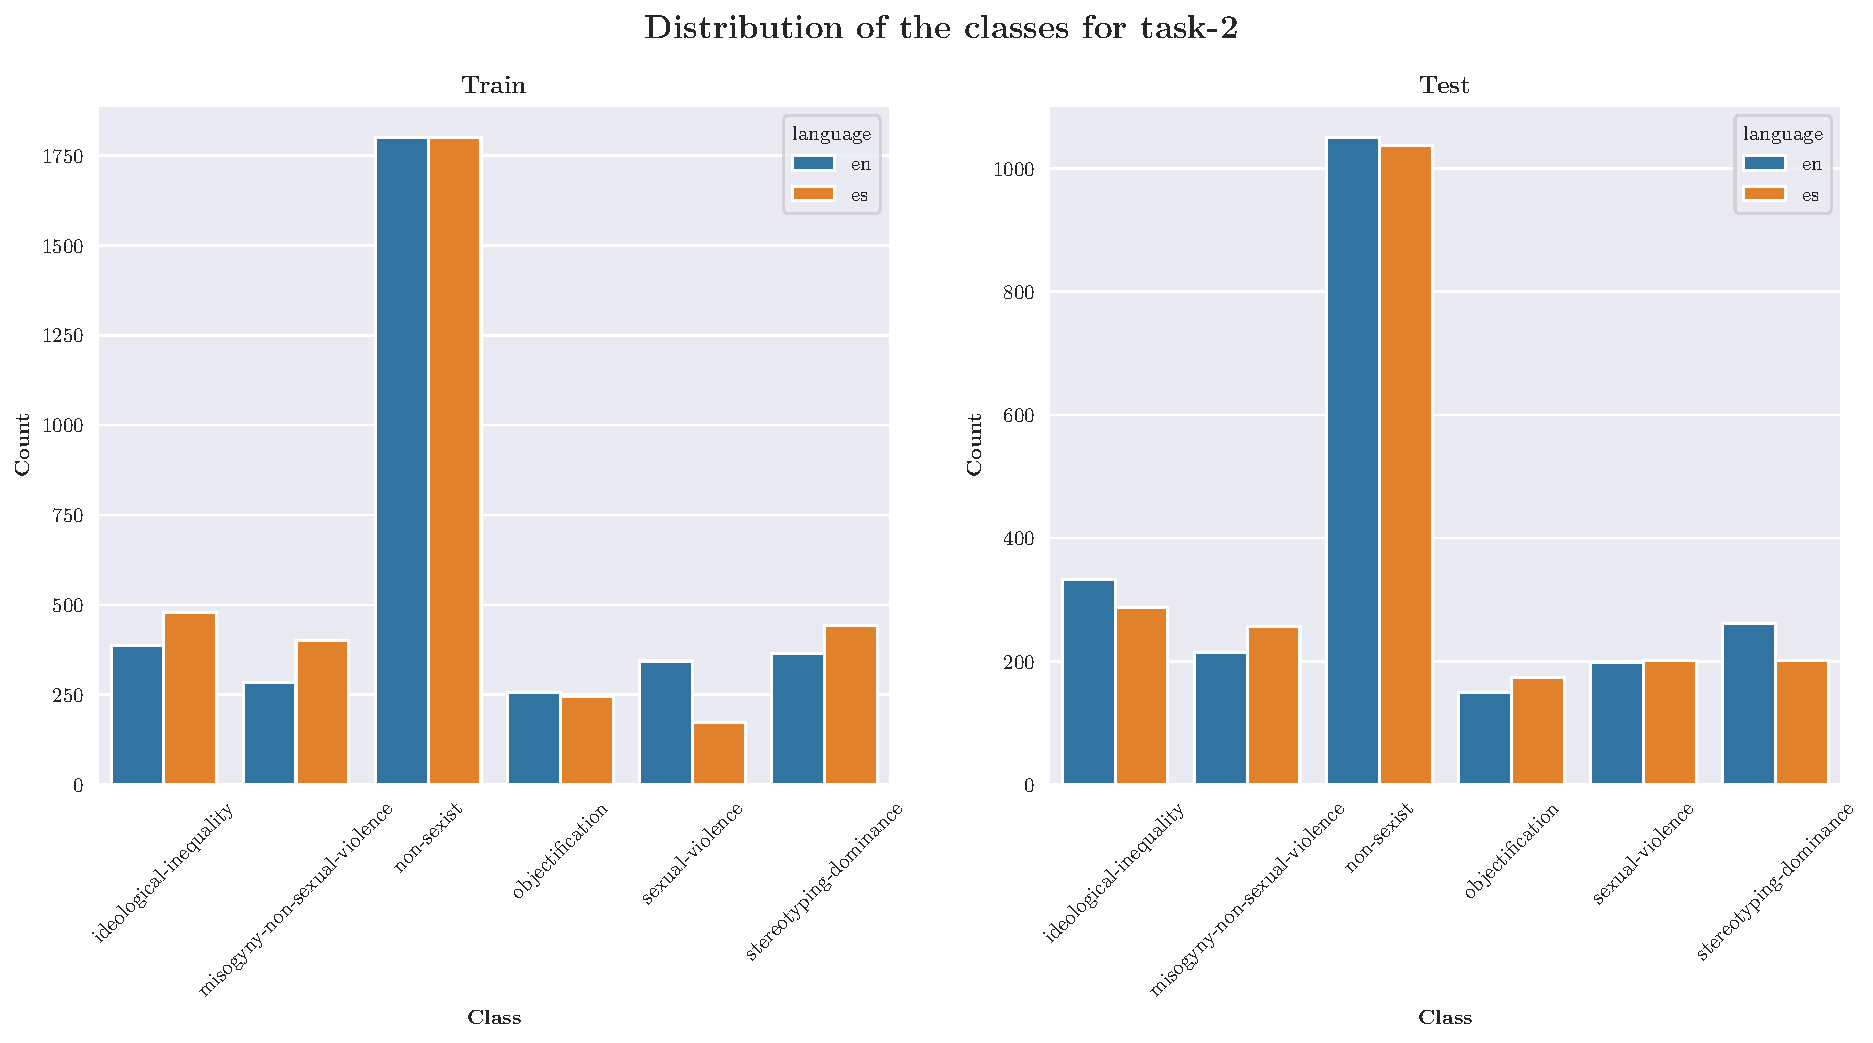
\includegraphics[width=0.8\linewidth]{images/task2.pdf}
\caption{Distribución de las clases en entrenamiento y prueba para la segunda tarea.}
\end{figure}

\end{frame} 

\section{Propuesta de solución}
\begin{frame}{Propuesta de solución}
\justify	
\small
\begin{enumerate}
\item Se hizo un pre-procesamiento simple del texto (pasar a minúsculas, quitar nombres de usuarios y urls), intentando además aplicar un spell-checker, ya que los textos de las redes sociales suelen contener muchos errores.

\item Se usaron distintos algoritmos para sacar características del texto, haciendo la distinción entre español e inglés, y se aplicó una regresión logística para hacer la clasificación en ambas tareas.

\item Su usó un modelo de BERT (\href{https://huggingface.co/bert-base-multilingual-uncased}{bert-base-multilingual-uncased}) entrenado en varios idiomas y una red neuronal para mejorar los resultados anteriores.
 
\end{enumerate}

\end{frame}

\section{Resultados}
\begin{frame}{Resultados tarea-1}
\justify	
\small

\begin{table}[H]
\centering
\resizebox{0.6\linewidth}{!}{%
\begin{tabular}{@{}cccc@{}}
\toprule
\multirow{2}{*}{\textbf{Modelo}}   & \multicolumn{3}{c}{\textbf{Task-1 (accuracy)}} \\ \cmidrule(l){2-4} 
                                   & Inglés         & Español        & Total        \\ \cmidrule(l){1-4}
tf-idf + LogisticRegression        & 70.70          & 69.81          & 70.26        \\
GloVe + LogisticRegression         & 66.35          & 67.82          & 67.08        \\
Doc2Vec + LogisticRegression       & 57.43          & 59.31          & 58.36        \\
sentence-BERT + LogisticRegression & 73.73          & 72.64          & 73.19        \\
BERT-base-multilingual-uncased     & 74.86          & 75.69          & 75.27        \\ \bottomrule
\end{tabular}%
}
\caption{Resultados para los distintos modelos para la primer tarea.}
\end{table}

\begin{figure}[H]
\centering
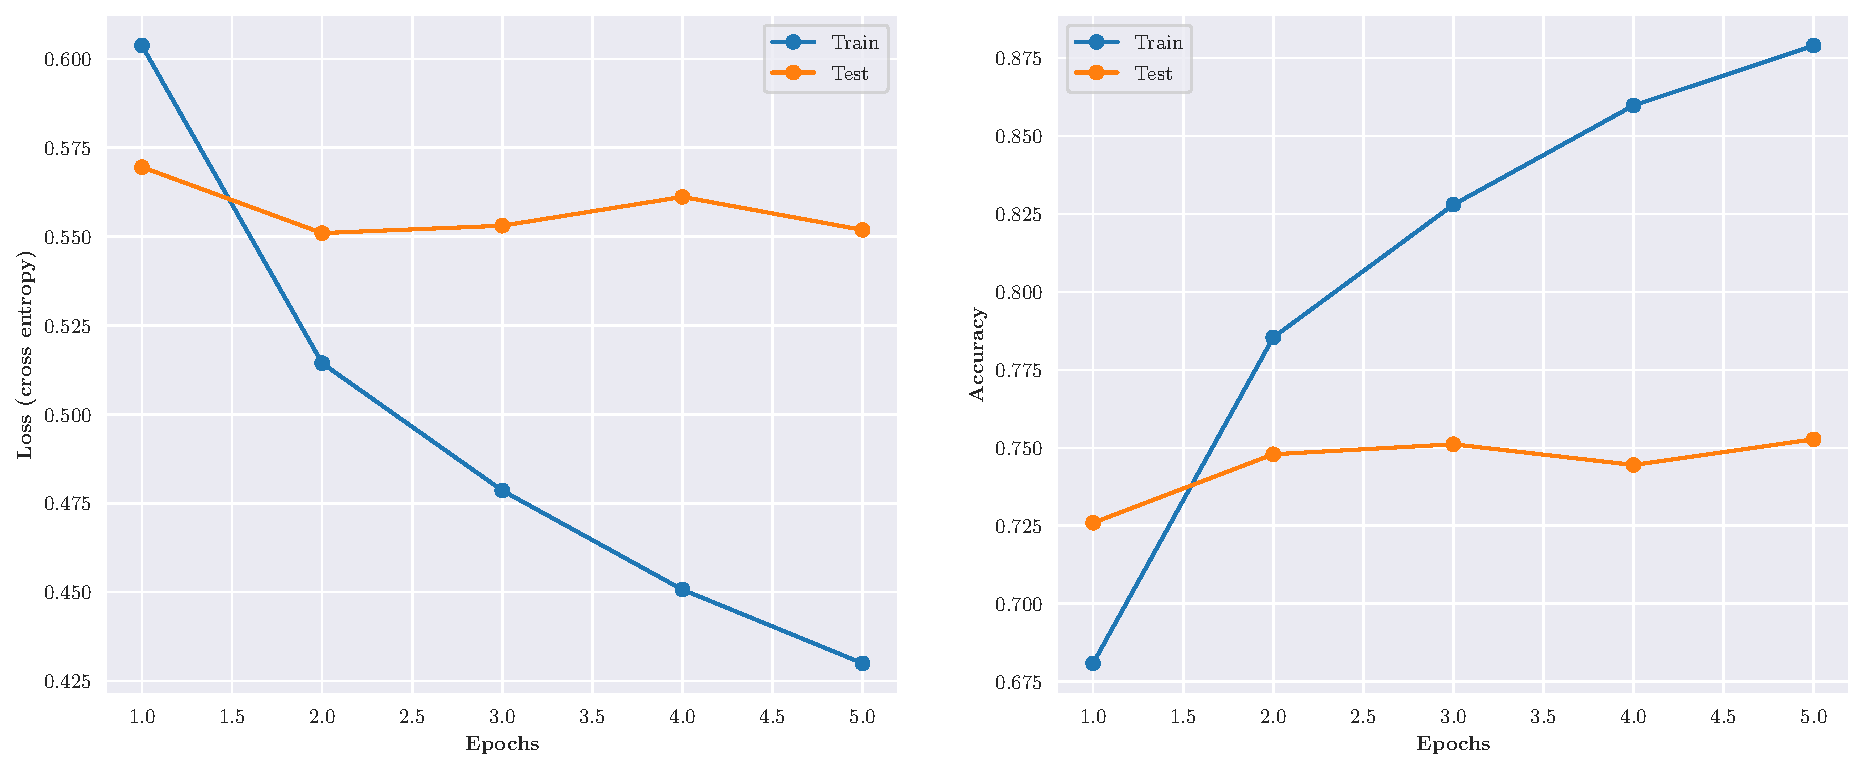
\includegraphics[width=0.6\linewidth]{images/BERT_tuning_task1.pdf}
\caption{Fine tuning de BERT-base-multilingual-uncased.}
\end{figure}

\end{frame}


\begin{frame}{Resultados tarea-2}
\justify	
\small
% Please add the following required packages to your document preamble:
% \usepackage{booktabs}
% \usepackage{multirow}
% \usepackage{graphicx}
\begin{table}[H]
\centering
\resizebox{0.6\textwidth}{!}{%
\begin{tabular}{@{}cccc@{}}
\toprule
\multirow{2}{*}{\textbf{Modelo}}   & \multicolumn{3}{c}{\textbf{Task-2 (F1 score)}} \\ \cmidrule(l){2-4} 
                                   & Inglés         & Español        & Total        \\ \cmidrule(l){1-4}
tf-idf + LogisticRegression        & 54.64          & 50.77          & 53.30        \\
GloVe + LogisticRegression         & 53.19          & 48.18          & 51.39        \\
Doc2Vec + LogisticRegression       & 38.18          & 37.87          & 38.41        \\
sentence-BERT + LogisticRegression & 59.99          & 61.08          & 60.76        \\
BERT-base-multilingual-uncased     & 61.67          & 62.95          & 62.38       \\ \bottomrule
\end{tabular}%
}
\caption{Resultados para los distintos modelos para la segunda tarea.}
\end{table}

\begin{figure}[H]
\centering
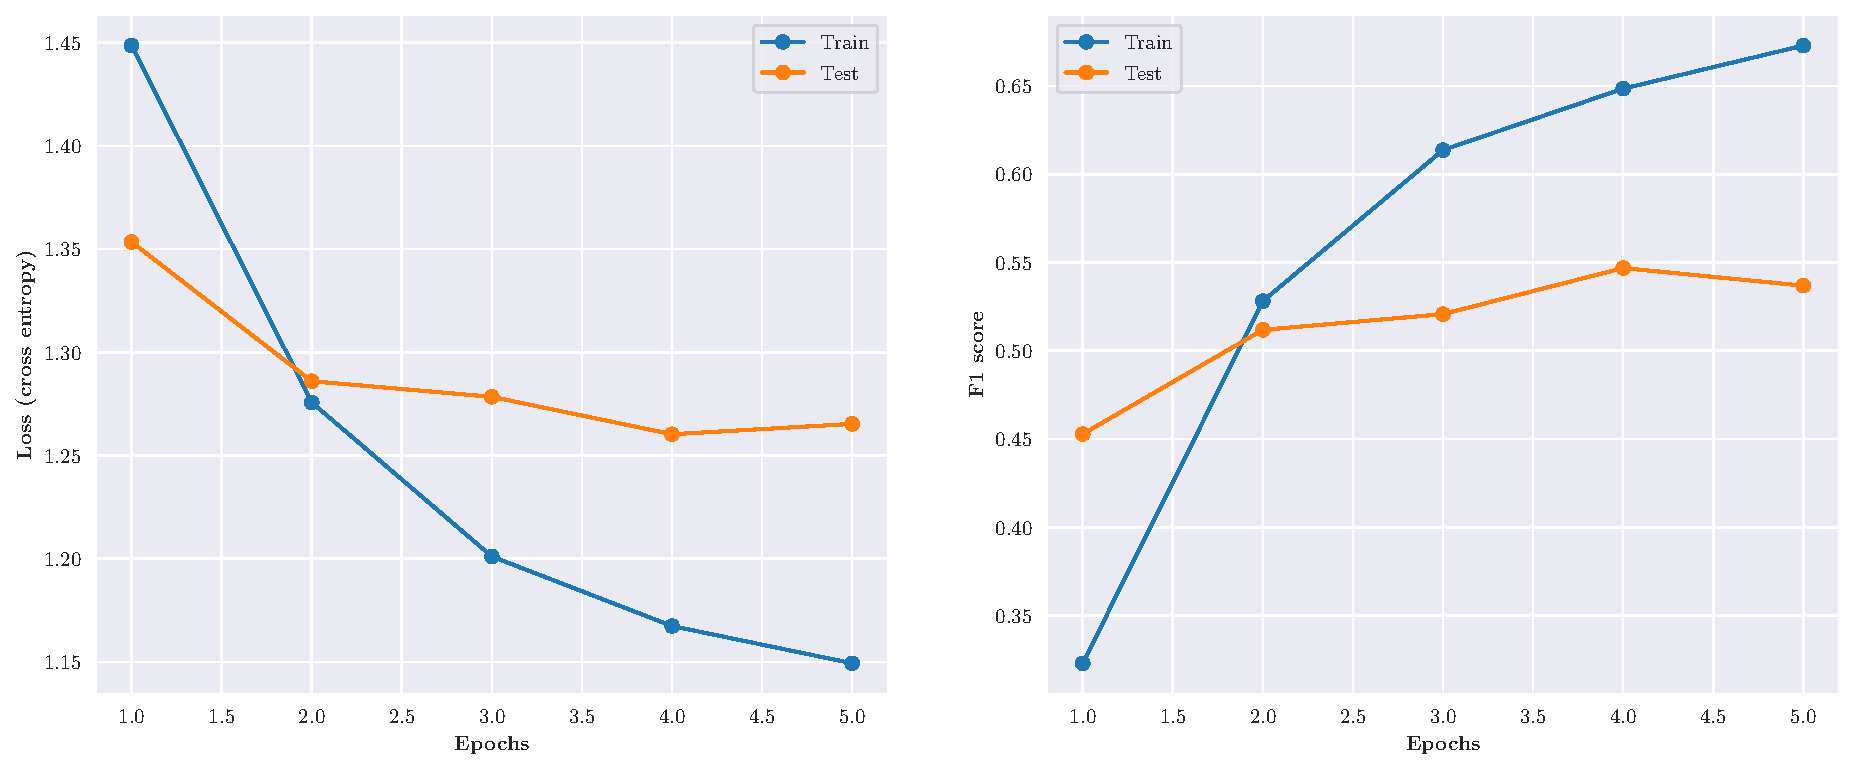
\includegraphics[width=0.6\linewidth]{images/BERT_tuning_task2.pdf}
\caption{Fine tuning de BERT-base-multilingual-uncased.}
\end{figure}

\end{frame}

\section{Conclusiones}
\begin{frame}{Conclusiones}
\justify	
\small

\begin{enumerate}
\item Observando los mejores resultados de la competencia, 78.04 de accuracy para la tarea 1 y 57.87 de F1 para la tarea 2, los modelos propuestos obtienen resultados sumamente cercanos, especialmente el que usa BERT-base-multilingual-uncased (75.27 y 62.38 respectivamente).

%\item Para la tarea 2 hay que usar primero el modelo de la tarea 1 y luego usar el modelo de la tarea 2 sobre aquellos que se predicen como sexistas, ya que yo sólo estoy usando un subconjunto de los datos para hacer la evaluación.

\item El spell-check debería funcionar para mejorar el pre-procesamiento, pero se debería usar un diccionario con el \emph{slang} de cada idioma para que de mejores resultados.
\end{enumerate}

\end{frame}

%\section{Bibliografía}
%\begin{frame}{Bibliografía}
%\justify
%
%\footnotesize{
%
%\begin{thebibliography}{00}
%\bibitem{goodfellow-2014}
%\emph{\href{https://arxiv.org/pdf/1412.6572.pdf}{Link Prediction Using Supervised Learning}}, Mohammad Hasan, Vineet Chaoji, Saeed Salem, Mohammed Javeed Zaki, 2006.
%
%\bibitem{dblp-dataset}
%\emph{\href{https://dblp.org/faq/1474679.html}{Digital Bibliography \& Library Project (DBLP) dataset}},  Schloss Dagstuhl.
%\end{thebibliography}
%}
%
%\end{frame}

\end{document}
